\documentclass[10pt,a4paper]{article}
\usepackage[latin1]{inputenc}
\usepackage{amsmath}
\usepackage{amsfonts}
\usepackage{amssymb}
\usepackage{makeidx}
\usepackage{graphicx}
\usepackage{url}
 
\usepackage{geometry}
\geometry{
	a4paper,
	total={170mm,257mm},
	left=20mm,
	top=20mm,
}

%\twocolumn

%opening
\title{\textbf{\Huge MimicVR \\
	\Large  Development of Human-Robot Interaction in Virtual Reality Space}}
\author{Santipab Tipparach, Keonwoo Kim, Daniel Ogburn\\
	\textbf{North Dakota State University}\\\textbf{Department of Computer Science}}

\begin{document}
\maketitle


\begin{abstract}

	The main goal of this project is to augment robot movement and decision making using the HTC Vive and a streamlined user interface. This paper will outline the history of virtual reality, why the Vive is the best choice, how robots sensory systems can be drastically improved using the lighthouse tracking system, and how robots and humans can better communicate by transmitting gestures and movement instructions through a virtual reality interface.

\end{abstract}

	\section*{Introduction}
	Virtual reality is a powerful tool in the worlds of data analysis and immersive simulations. The HTC Vive introduces a method of entering virtual reality and capturing a user's precise movements. This is all possible using the HTC Vive's light house technology, which provides sub-millimeter positional accuracy. There has been some work already done introducing robots to the virtual world, however this project takes some of the projects found online and takes it a step further. On the website Hackaday.com, many projects are outlined \cite{hack1}. This includes a project that was very like our initial setup, however the project on the website was a very small scope and was surpassed by this project on the first weekend. Another project demonstrated the power of augmentation by tracking a drone in a virtual space and using this technology to swap batteries quickly on a base and fly for another fifteen minutes. This project will utilize the Vive tool, the Elegoo robot kit, and a central CPU/GPU to render, simulate, and send instructions via Bluetooth from a virtual environment to the physical robot.

	\section*{Background}
	In the past, robots used various techniques for tracking and motion sensors such as line tracking, IMU(Inertia Measurement Unity), ultra sonic, and various methods for sampling points with depth. One of the biggest challenges of positional tracking is that the positional coordinates of each tracked object is best used in relation to another object, it becomes difficult for the tracked object to work on it's own by only sensing the environment.
	\\\\
	In GPS technology, an array of satellites orbit the earth to help triangulate a position in a 3D spatial coordinate system using the time differences each satellite is from the center point \cite{gizmodo1}. For a very long time, the few feet of inaccuracy was tolerated for large scale navigation (moving over vast distances of miles). However, when it comes to tracking at the finer scale, the human scale, we cannot use GPS for close range, high precision tracking.
	\\\\
	The HTC Vive, released in April 2016 \cite{techradar1}, provides room scale tracking with high accuracy. Mainly used for Virtual Reality, this project will utilize this advantage to harness that accuracy into encoding instructions and providing robots with human like tasks. Upon solving the issues of precision, simulations can be designed and algorithms can be tested all using the virtual space.
	\\\\
	In addition to high accuracy tracking, VR also allows for a safe and cost effective space for testing out various situations for robotic behaviors. An example of this maybe in a hazardous environment\cite{Bugalia} with lethal radiation or a potential bomb threat\cite{Codd-Downey}. This main reason alone, combined with certain time critical tasks can utilize the power of VR not only to simulate, but allow operators to interface with the robot in realtime in a safe environment. Long past are the days of joystick controls for operating analog robots. With the advent of VR controls, robots not only mimic human behavior but can actually learn to do better than their human counter parts and in turn, humans can learn from those robots as well.
	
	\section*{Description}
	The aim of this study is to develop an infrastructure and show how a robot or autonomous agent can have a centralized control system in a remote location and be able to operate in real time using data collected from the environment.
	\\\\
	The purpose of this is to collect data and analyze possible movement choices or decisions in realtime using a large CPU. Once the Vive tracking system is able to triangulate movement, the cars then have an accurate position data represented in VR. This in turn allows the computer to figure out various factors to feed to the actuators. Data will include rotation speed, movement speed, which can then provide data on friction and roughness of the environment.
	\\
	All this allows the system to adjust to various environments and allows it to figure out how to complete a goal optimally.
	\section*{System Description}
	The following is a high level system architecture and of how the simulation API and communication system works.
	\begin{figure}[h]	\centering
		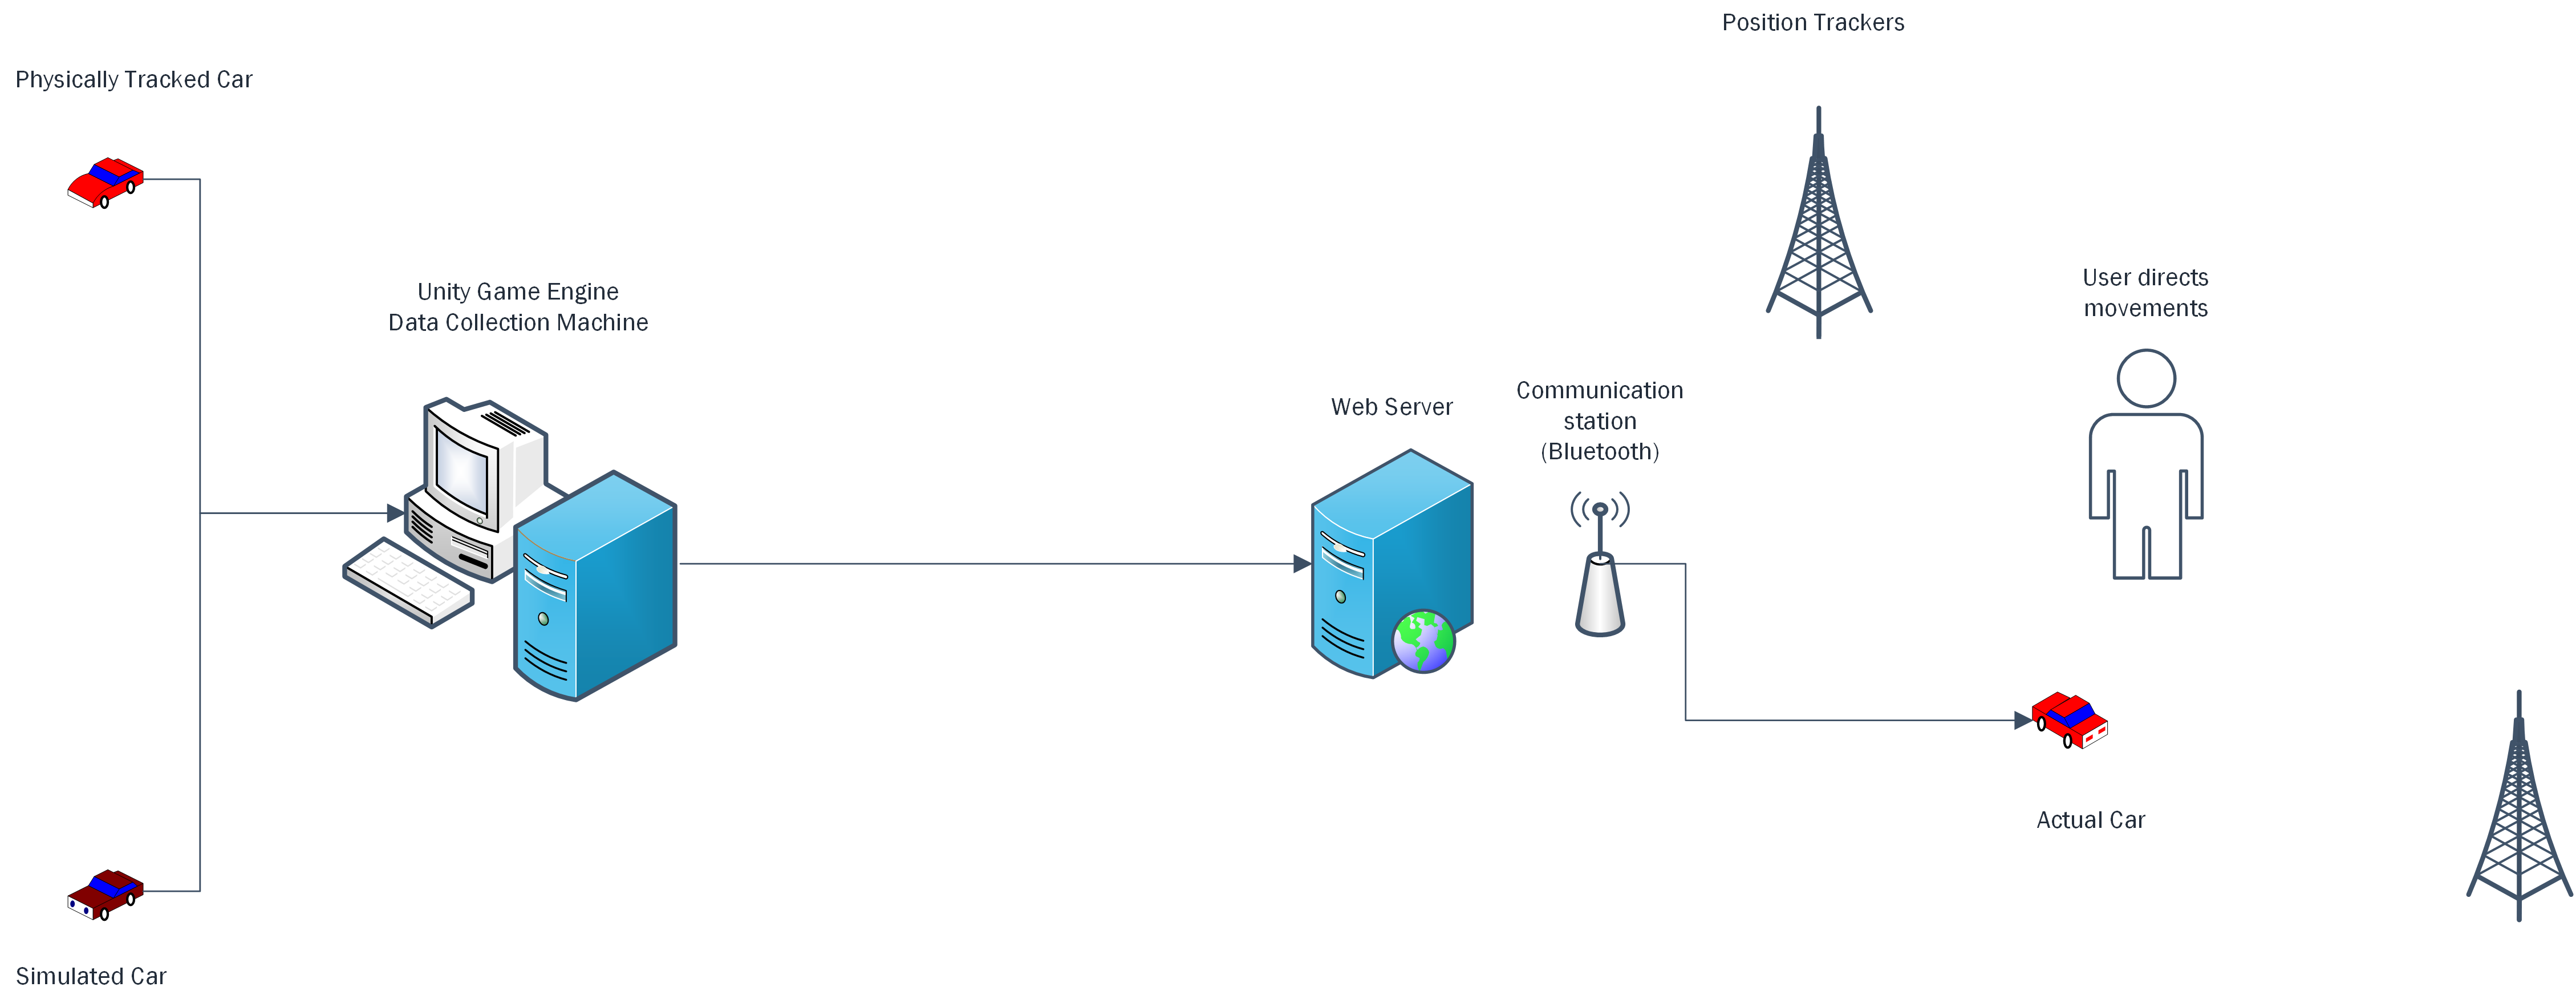
\includegraphics[width=1\textwidth]{AwesomeDrawing.png}
		\caption{The high level network architecture of showing how the virtual and physical cars implement the same algorithm using a common API.}
		\label{fig:system-architecture}
	\end{figure}

	In figure \ref{fig:system-architecture} the agent is the "actual car" on the far right. The two left cars are simulated in the Unity game engine as seen in figure \ref{fig:robot-rivalry}. The user directs the car where it needs to go, the tracking systems pick up the car's location and orientation in 3D space and relay that information back to the main computer which hosts a running instance of the Unity Game Engine.
	\\
	This data is then used to update the game engine's virtual representation of the physical car. As the simulated and tracked cars use the same code, they both hold the API with different actual implementations. The tracked car holds only the code to synchronize its position and rotation, while the simulation car holds code to actually apply force to the rigid body physics model inside the game. The main difference is that the tracked car object actually holds a network interface as well that forwards any instructions made in the game engine to the physical car model. This is what drives the agent to move.
	\\
	The user is then able to issue commands to the car either remotely at the location of the physical car, from the computer with the game engine, or in any other location that has a connection to the web server that is connected to the physical car.
	\section*{Overview}
	This study examines the use of VR as an interface tool for robotics. The main question here is, how can Virtual Reality technology be used to augment the simulation and command of physical robots? The environment will be set up in Unity with the SteamVR software installed. It is also using the VR toolkit from the Unity asset store.
	\\ 
	To simulate robotic systems, a Unity rigid body object is assigned to a simulated version. 		\begin{figure}[h]
		\centering
		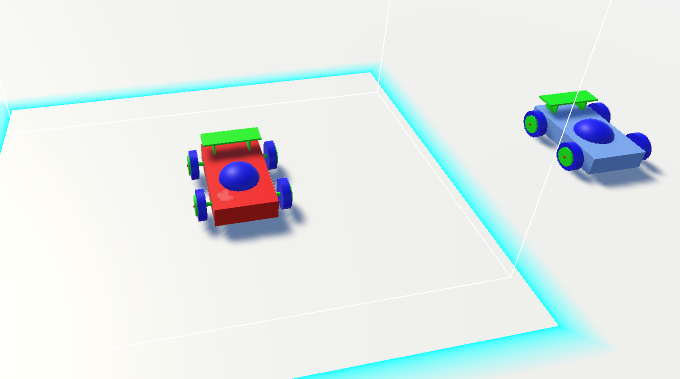
\includegraphics[width=.4\textwidth]{robot-rivalry.png}
		\caption{Two robots competing to execute behavioral algorithms, the physical (left) and the virtual (right).}
		\label{fig:robot-rivalry}
	\end{figure}
	The main implementation feature of the project will be the simulation code. With the infrastructure to relay data from the positional tracker from the robot to the desktop, and the desktop runs a simulation that will send back data, a script can be quickly written to provide different behavior systems to run using a secondary tracker.
	\\ 
	Basic instructions can be encoded such as moving in a circular motion once, and then will be translated to both robot models, the physical and virtual simultaneously. This allows for data collection and analysis of the difference in the algorithm used for the physical and virtual counterparts. In addition data can be collected in terms of delta-rotational and delta-velocities to determine correct orientation and speed using timed outputs of movement commands.
	\\ 
	This feedback loop is ideal for a continuous course correction algorithm. The code will adjust rotation to the desired direction vector, and a forward/backward drive will move the car to reach its target. If it passes, it will move back and adjust itself until it is with in acceptable bounds. This will allow the robots to hit targeted way points without any external guidance.
	\\ 
	Experiments will be designed to test out various user-to-robot interfaces such as commanding the robot to follow a designated way point. Sets of different waypoints will be used to test the PID systems, and other implementations if needed. Some adaptive learning techniques maybe applied so that the robot can calibrate itself on various terrains.
	\\ 
	The first stage of experiments will be to test out the capability of following multiple way points in 2 dimensional space. These will include, single way point navigation, multiple way point navigation, and simulated collision avoidance.
	\\ 
	The second stage of experiments will be designed to test out 3 dimensional movements. While this will still be used on a wheeled robot, the robots will still have portions in the simulation that can move in the Y-Axis (Unity uses the left hand coordinate system with Y as up/down). This should allow a robot to follow the movements of the secondary tracked object with high precision using the navigation and path finding system and the high accuracy tracking system of the Vive.
	
	\section*{Implementation}
	From the very start, an iterative approach to developing the system was taken. For each week, sometimes two week period the team would meet on a Sunday where everyone was available and figure out a way to sprint to the most viable goal within a 3-4 hour period. At first, a robot was assembled with the kit provided. Then the implementation began to develop a tracking system.
	\\
	The very first iteration of this was the Mimic MK1 (figure \ref{fig:mimic-mk1}). The first model was meant to showcase a proof of concept as to how the robot would be tracked in virtual space. At first, there were some complications with getting the robot's rotational offset to track correctly, but it was quickly resolved by setting a time delay, allowing time for the Vive to sync with the controller's position and orientation. After that the tracked position of the robot was near perfect.
	\\
	Next up was the communication. Clearly, the work flow was exhausting to write code and upload to the system was tedious. This meant less time actually testing out code logic, and more time fidgeting with the compile and execution process. So the decision was made early to offload all the logic to the desktop computer, while maintaining only basic instructions on the robot. Luckily a script with basic controls for bluetooth serialization was available out of the box, and the with some minor modifications, it was installed in the robot for a quick proof of concept.
		
	\begin{figure}
		\centering
		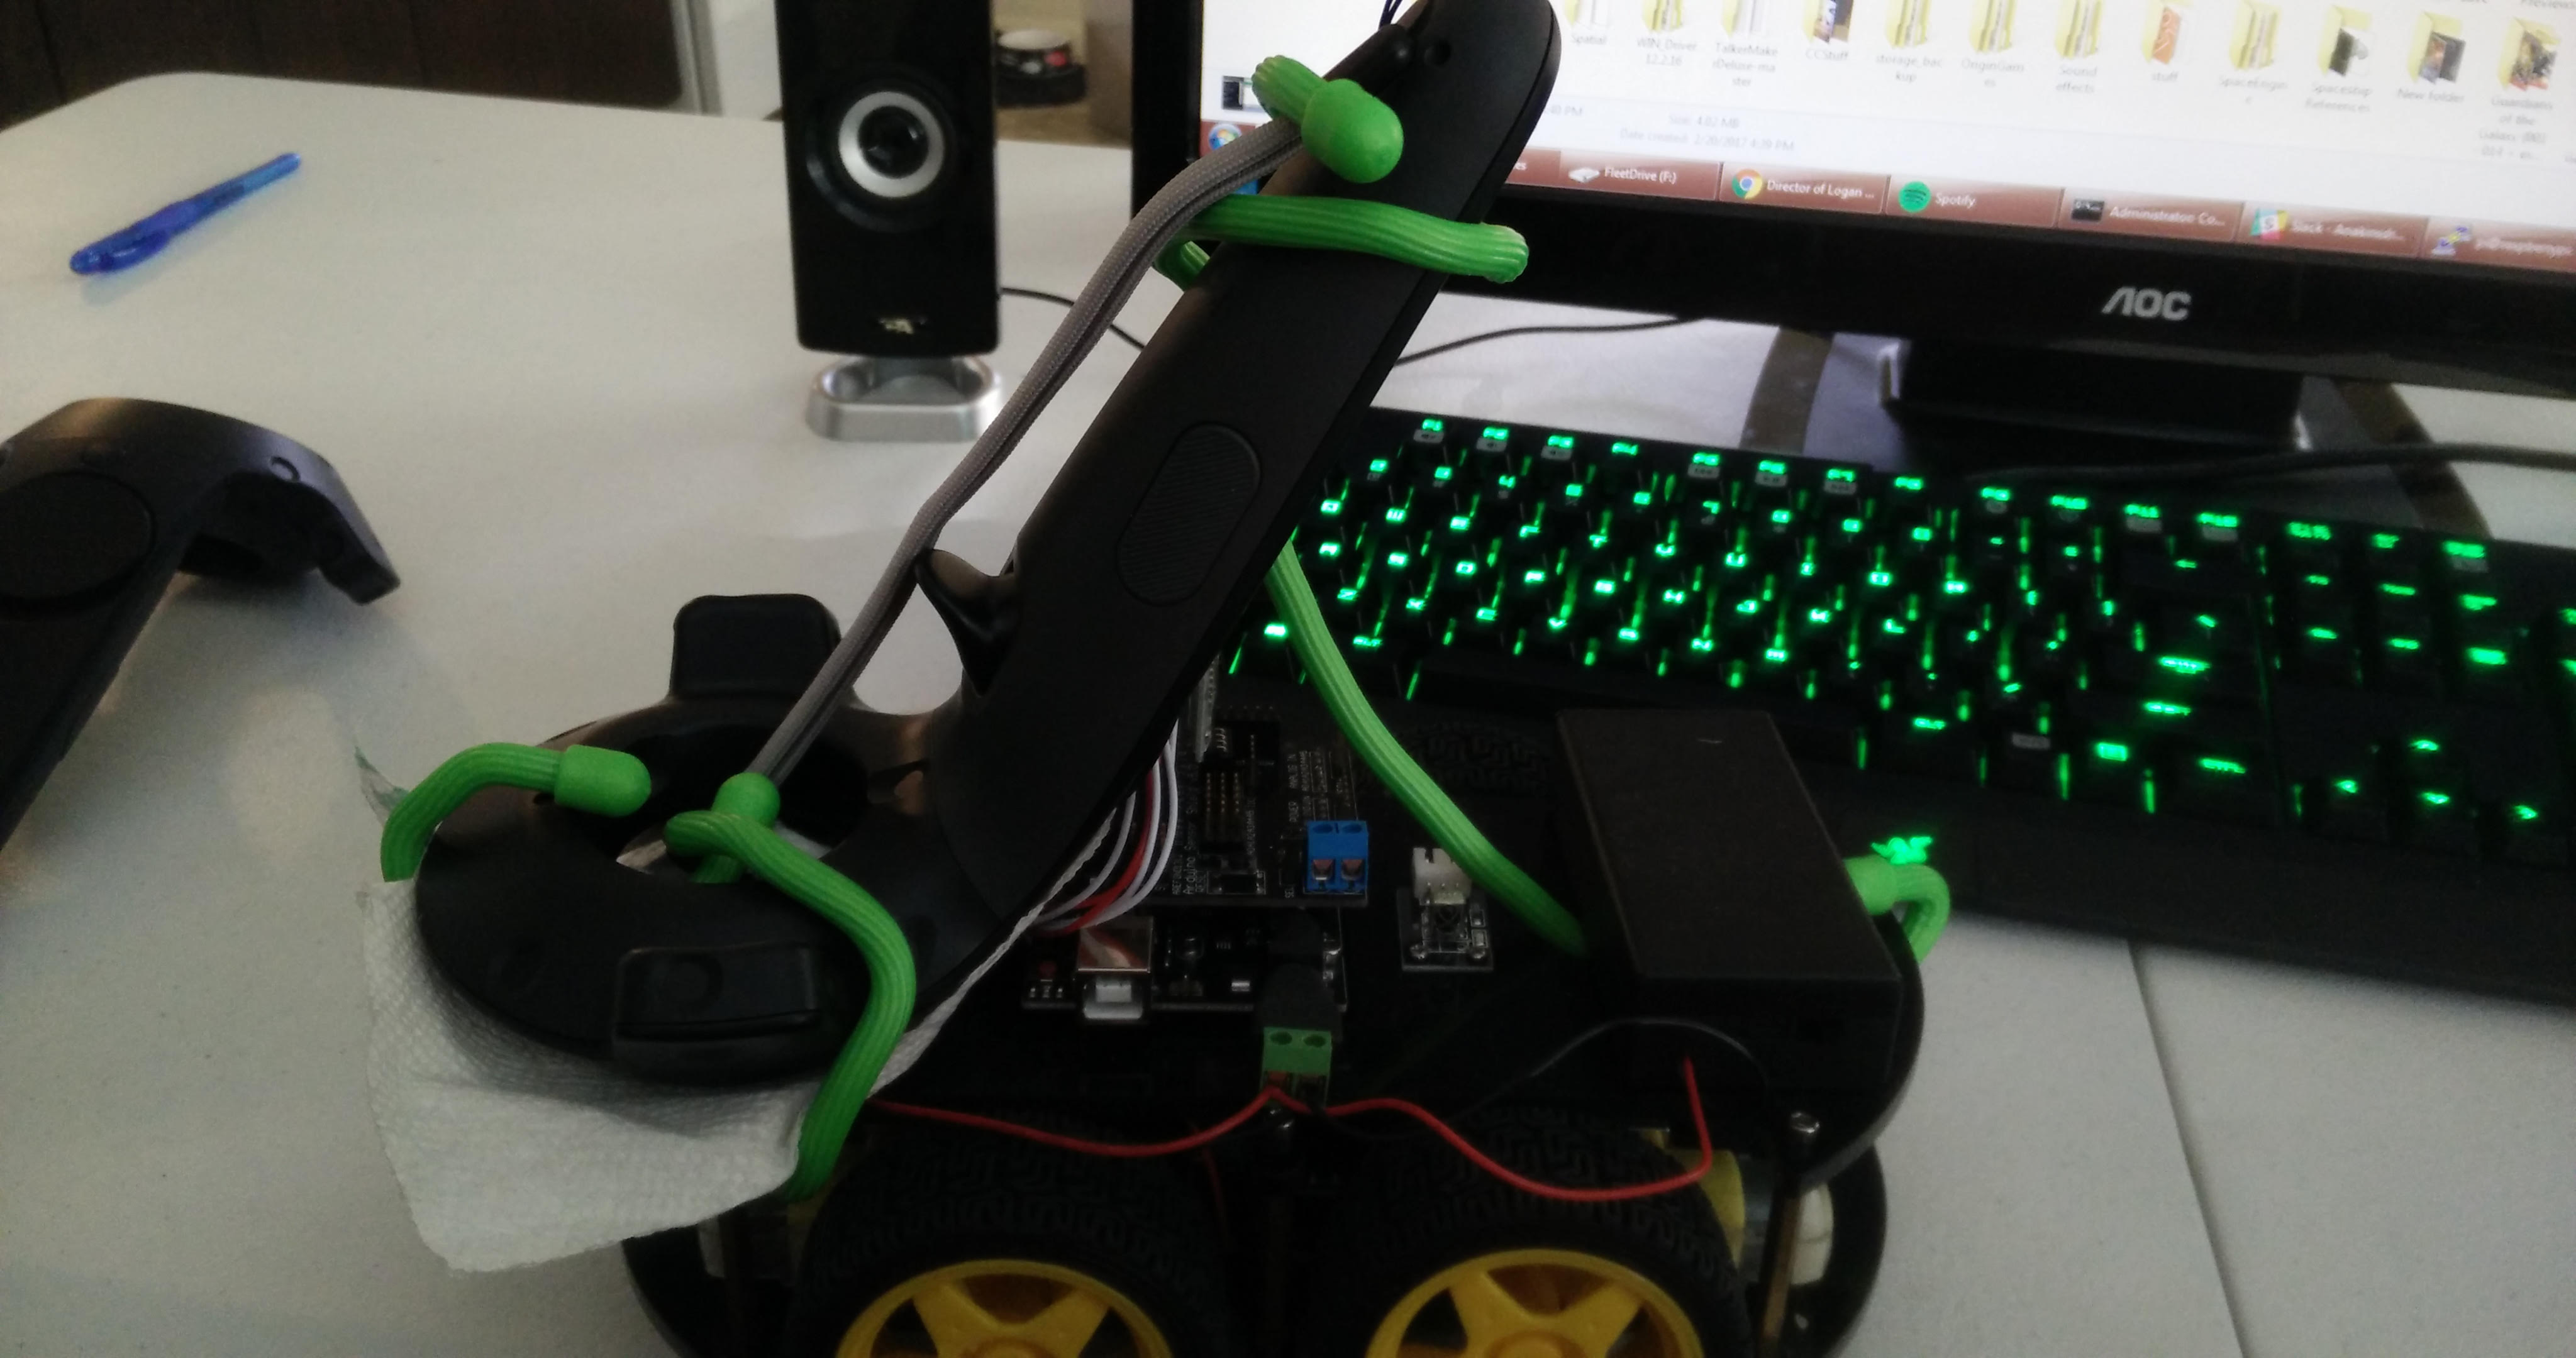
\includegraphics[width=.6\textwidth]{robotv1.jpg}
		\caption{Using a hand controller and gear ties to mount onto the robot.}
		\label{fig:mimic-mk1}
	\end{figure}
	
	The next stage of MK 1 was to develop an automated communication system. Although position was being provided, and now uploading of information from the robot was required (since the tracked objects took care of that), only data needed to flow one way from the desktop to the robot's bluetooth receiver. Unfortunately, the desktop being used was not working with bluetooth, a workaround done to use a persistently running Raspberry Pi. Mounted to one of the light house(Vive's tracking system uses a laser sweep module at 2 corners of a diagonal of the room) fixtures, the Pi was able to operate out of site and out of mind. There were some troubles installing Pi software that would enable bluetooth with the language of choice, Node JS, but eventually a suitable bluetooth package was found and data was able to be streamed directly from desktop to Pi and finally to the robot.
	\\
	After getting communication set up via Node JS application servers, a logic script had to be tested. The choice of this was Unity 3D. Because unity 3D had VR capabilities built into already, a simple installation of SteamVR SDK and the VR toolkit were all that was required to get the system running. However, Unity still needed to communicate with the Node JS server, so Socket.io was installed into Unity. Although no longer supported, and outdated by a few years it did the job. Perhaps in the future a switch to an officially maintained distributable version of socket.io would prove more useful when it comes time to implement more advanced networking protocols. Once the communication from Unity was setup, a direct line went from the Unity editor all the way to the robot. With the implementation of a simple control API, a simulation robot and the VR controlled robot could execute the exact same code but control two different systems. One being the simulated physics system in Unity and the other being the actuators on the robot. Hence the robots are mimicking one another.

	\begin{figure}
	\centering
	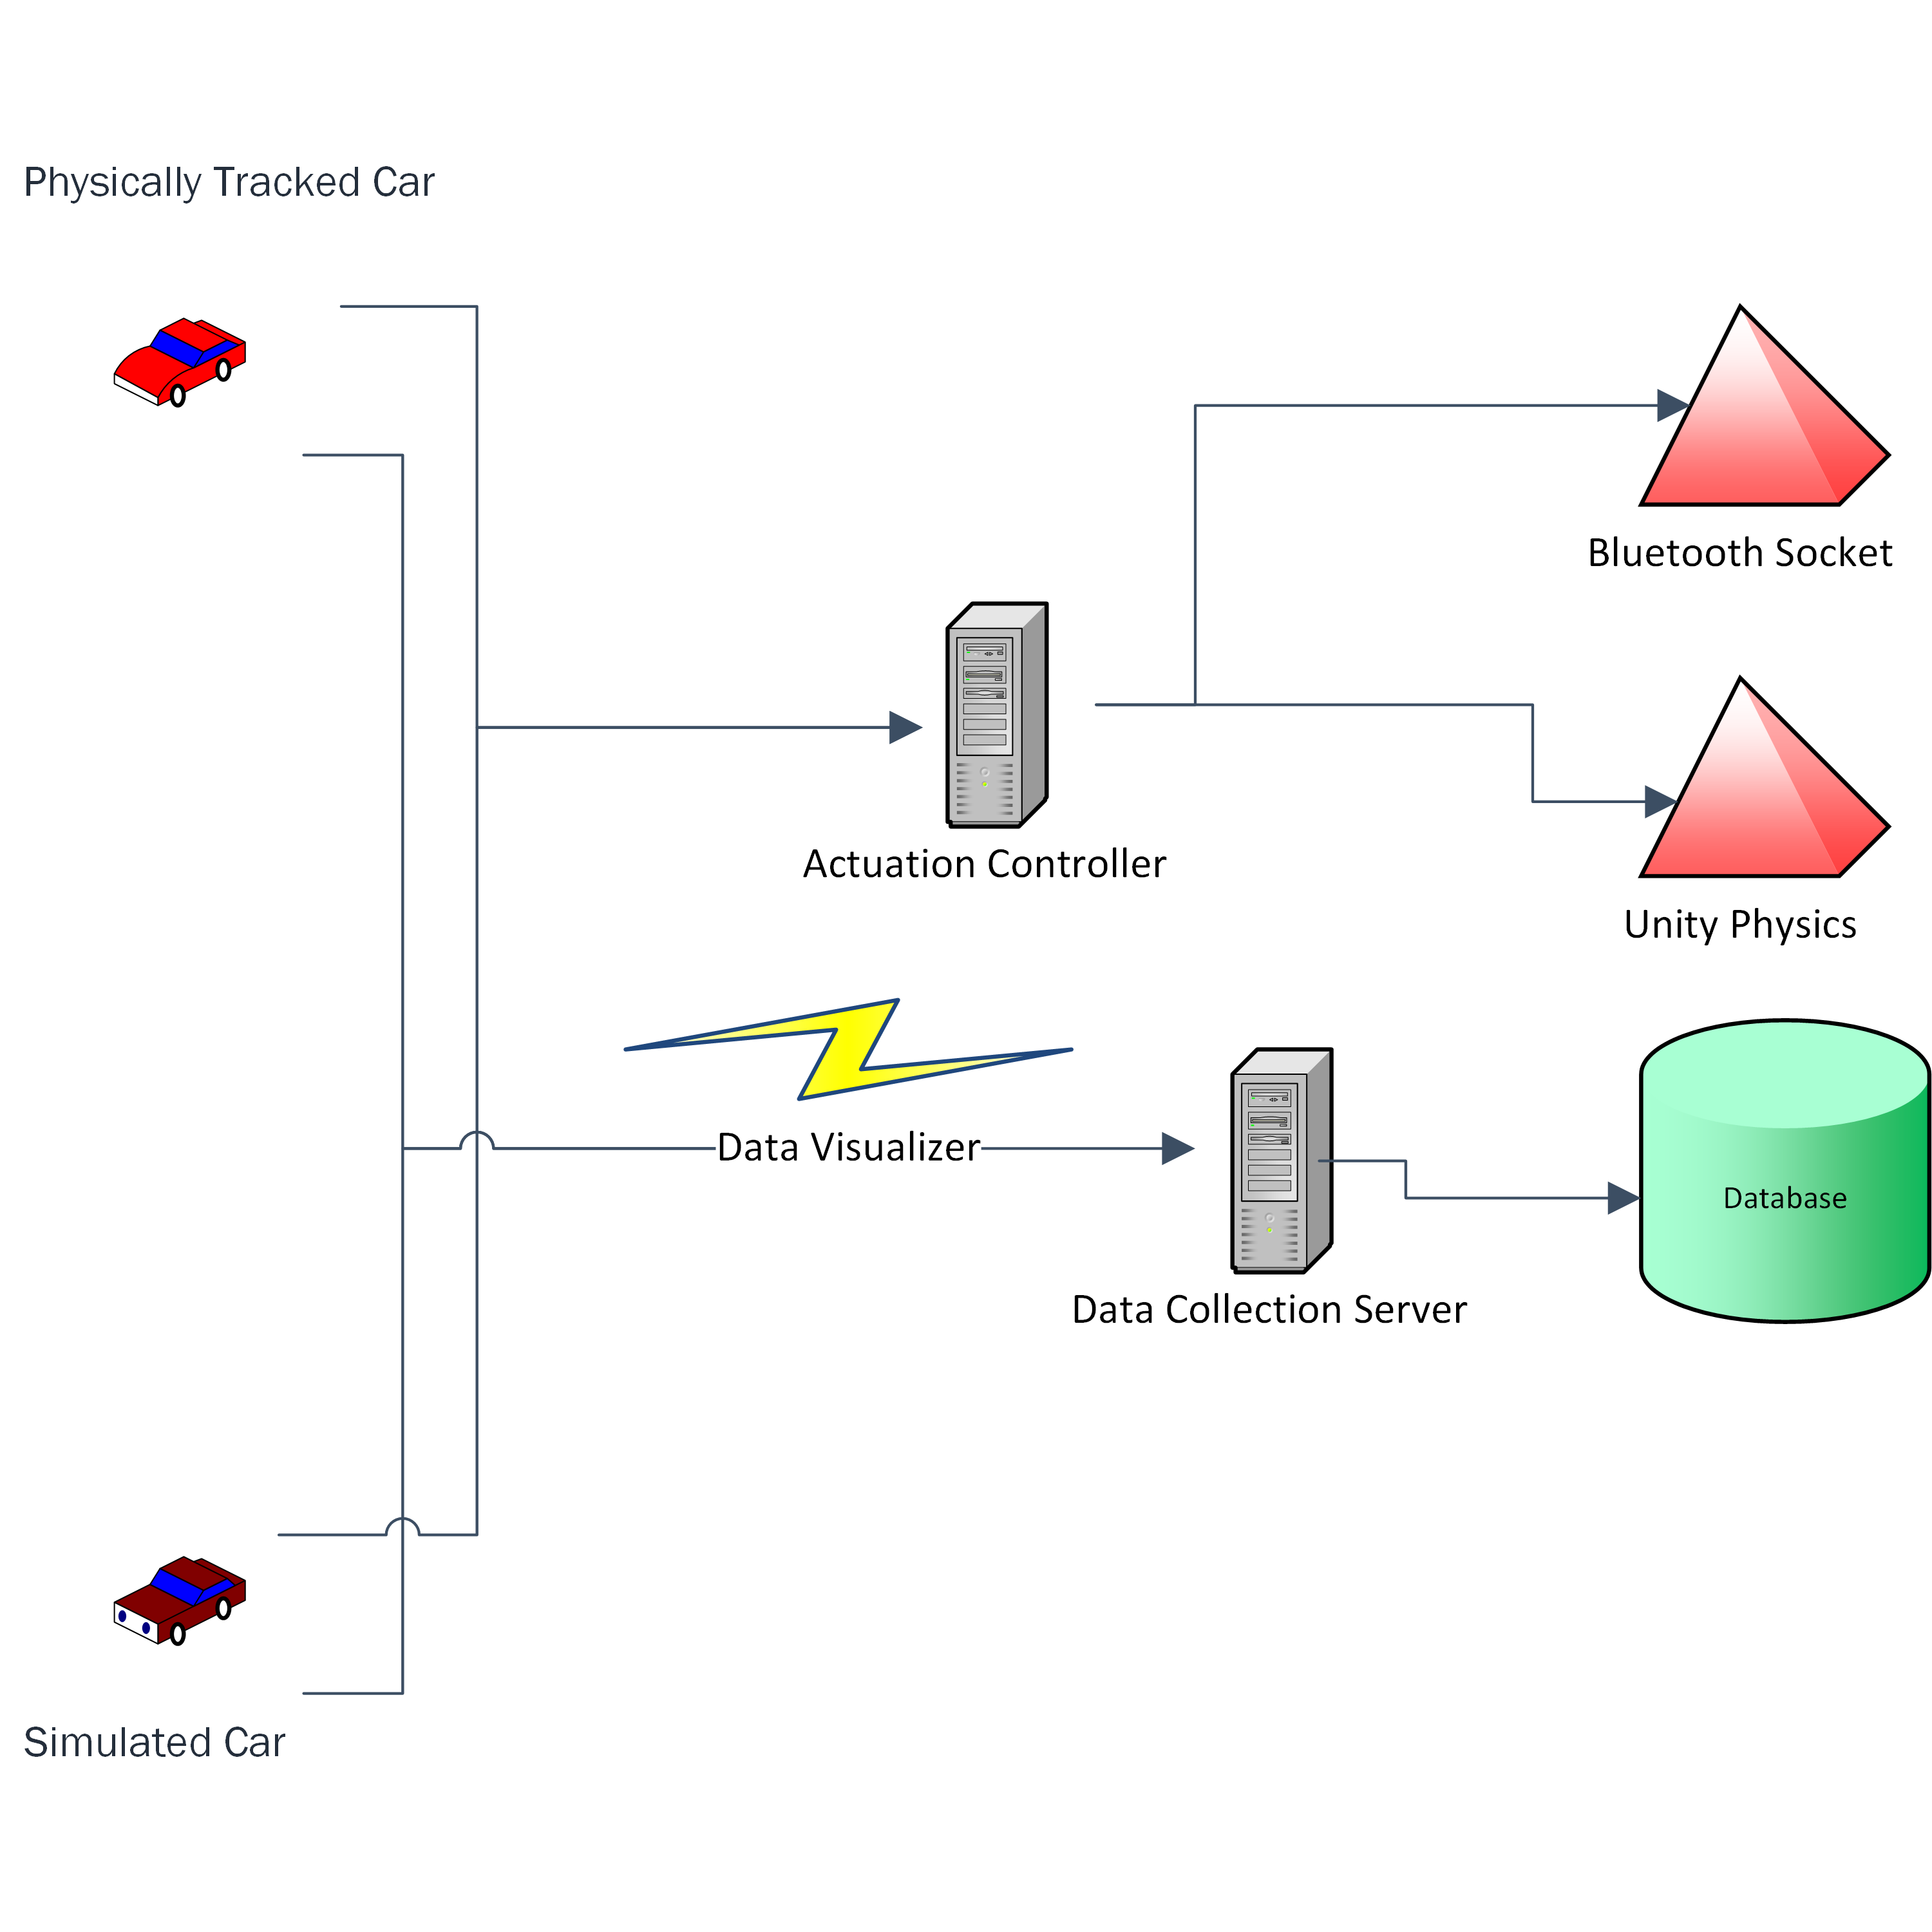
\includegraphics[width=.6\textwidth]{Network_pipline.png}
	\caption{Detailed look at the network portion of the architecture.}
	\label{fig:network-pipe}
	\end{figure}

	Once this phase was complete, the next phase would no longer involve physically altering the robot or the VR system until the official Vive tracker would be released. For the next stage, a few iterations were taken to experiment on possible control schemes for driving the simulation and physical robots. Because the simulation had to strictly follow the behavior of the robot vehicle restrictions such as certain force, translation, or rotation operations were strictly prohibited. In fact, only the forward, backward, left, right, and stop instructions were coded into the simulation robot. The first iteration of this code was to use a variable timed interval to command the robot to move. For example, if it took 2 seconds to turn right 90 degrees, this command would be fed into the robot beforehand and wait 2 seconds until the next command. There were a couple of problems with this approach. The first was that neither the model or the actual robot were deterministic. This meant the time it took to rotate or move were not always fully predictable. This led to lots of cascading failures, where a miscalculation of rotation interval spiraled into the robot being stuck in perpetual rotation that were never near its intended target. Then the next approach was decided on, it turns out that the system ran much better without the timed instructions, but with incremental instructions. This allowed the robot to behave more like a responsive agent. This meant that any protrusion such as changes in floor friction or external changes in course would be quickly corrected. Unfortunately, the bluetooth system could not fully exploit this feature due to the delay between the web socket and bluetooth layers. However at 5-10 intervals per second, or roughly 100-200 milliseconds, the instructions were able to make it through well enough. Thus the max number of instructions sent was 10 times per second.
	
	\begin{figure}
		\centering
		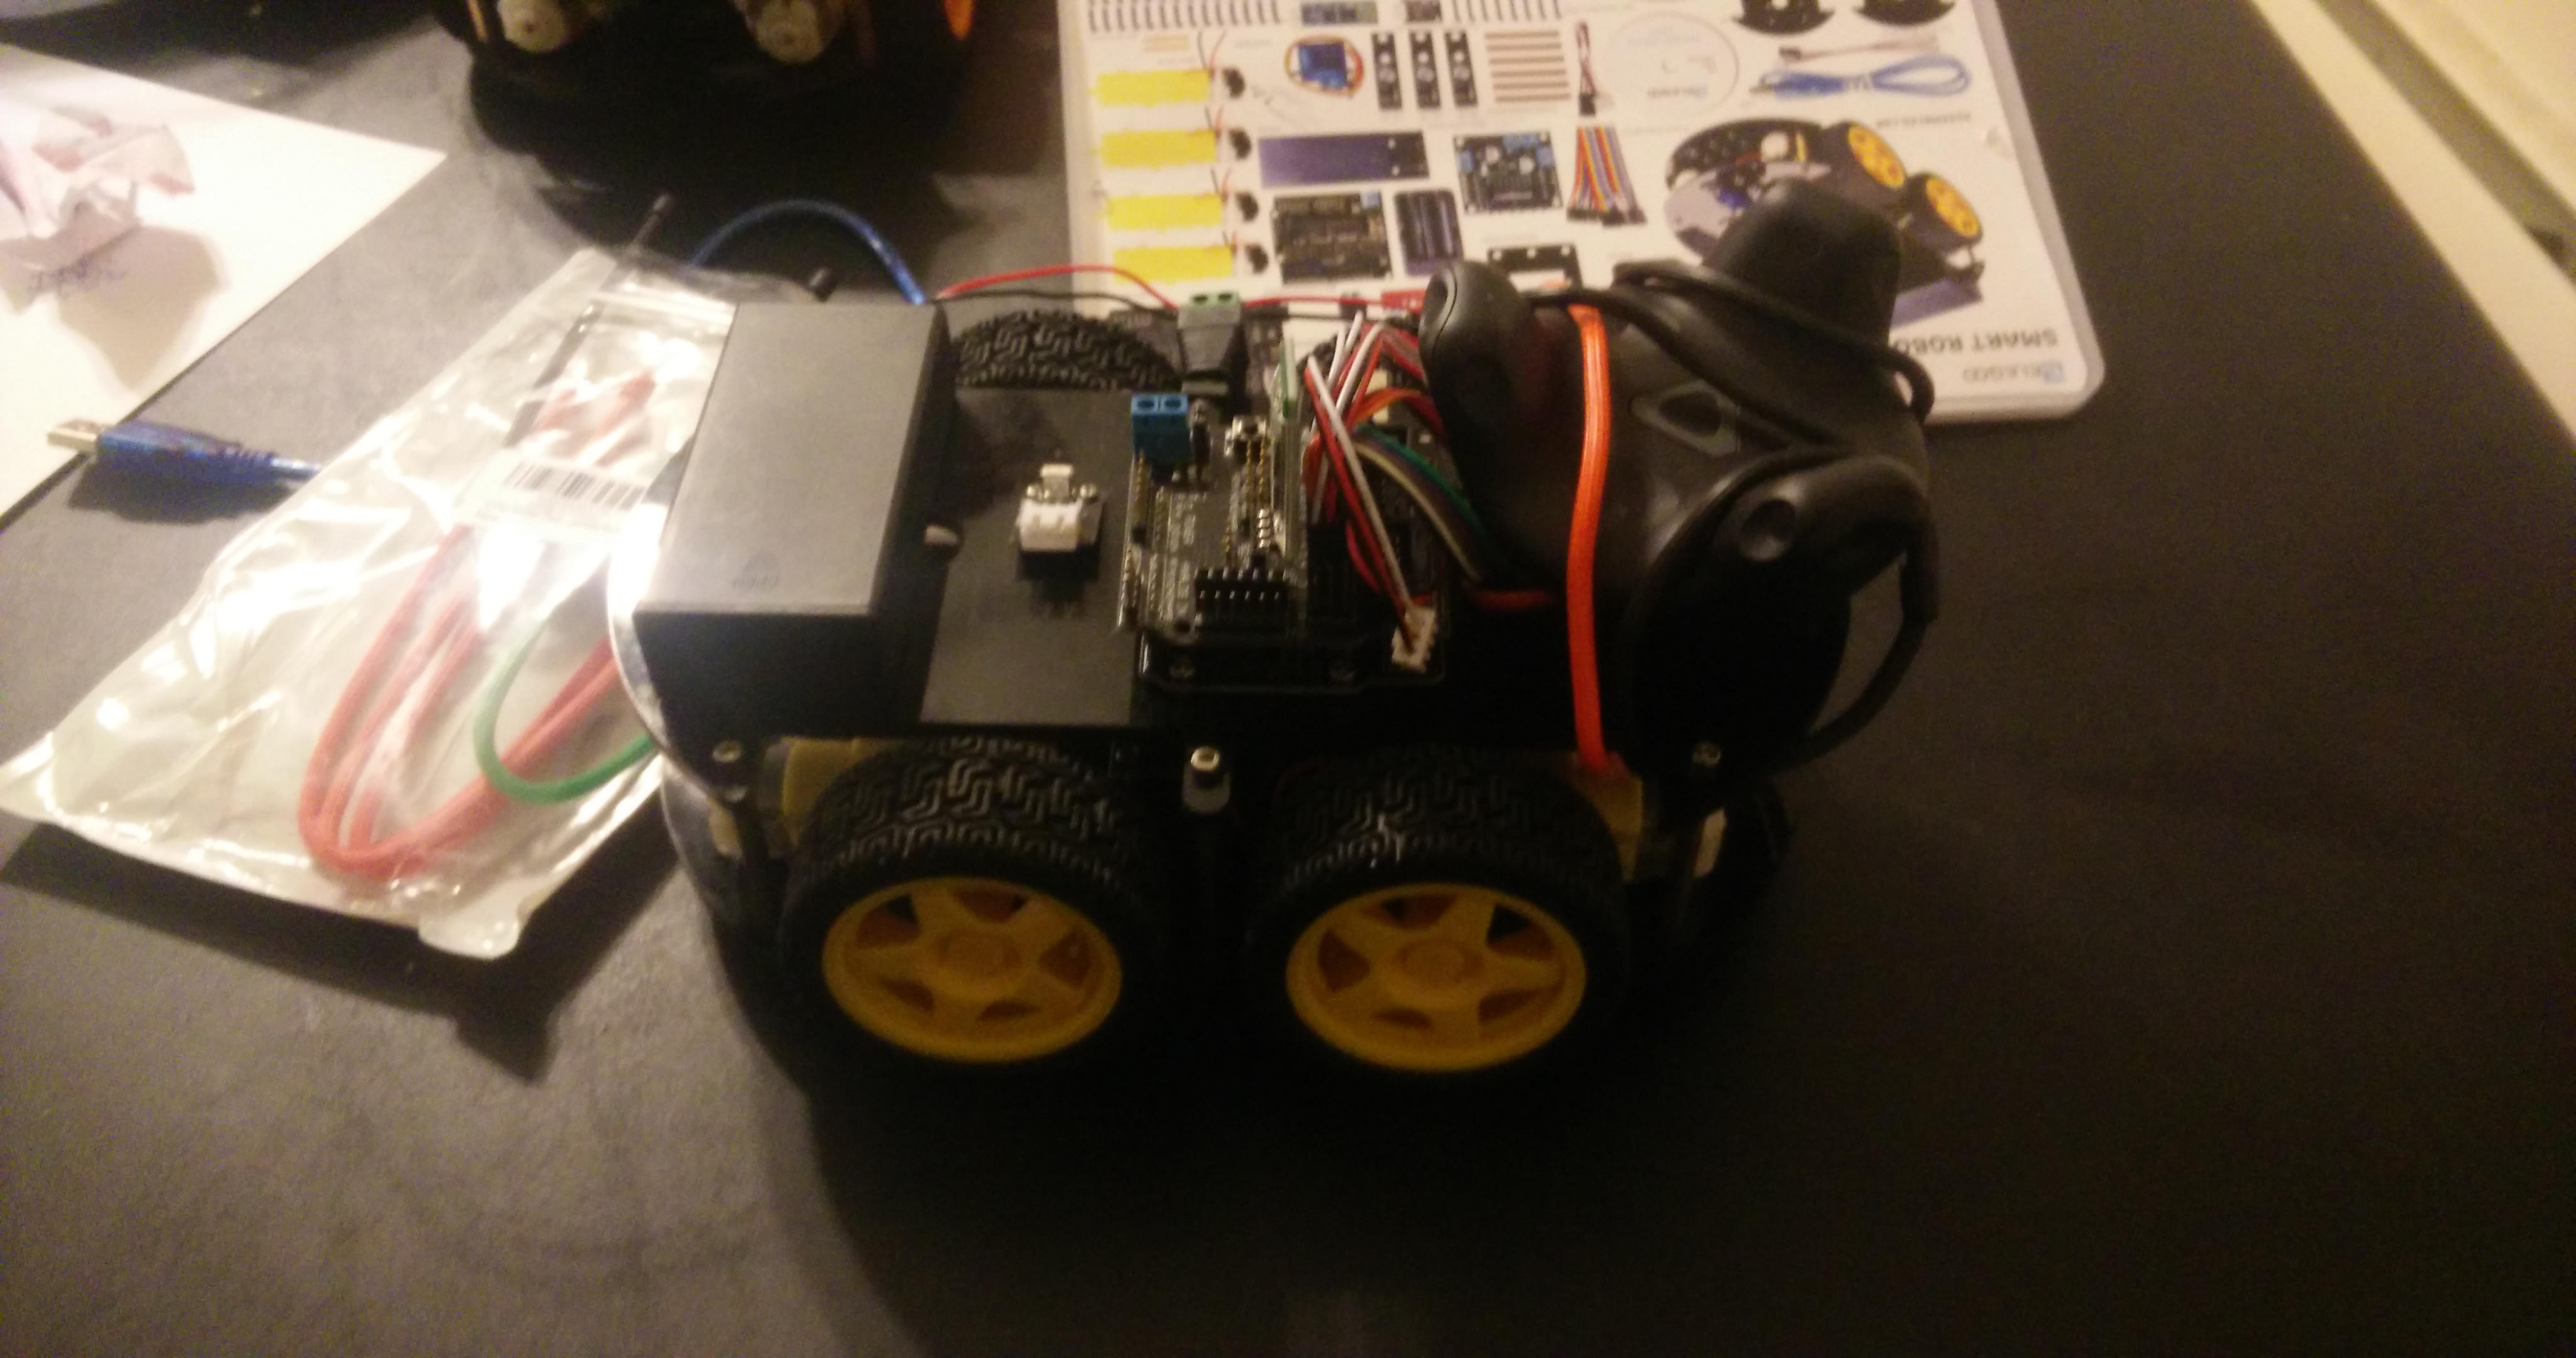
\includegraphics[width=.6\textwidth]{robotv2.jpg}
		\caption{Much lighter in weight, the MK2 allowed for a much more stable mount, and there was no more need for the delayed tracking, since the orientation of the tracker device was always the same as the robot.}
		\label{fig:mimic-mk2}
	\end{figure}
	
	By this time, the Vive tracker had arrived, and it was time to retire the clunky, unstable hand controller on the robot. Enter the Mimic MK 2 (figure \ref{fig:mimic-mk2}). This version will run on the new code developed almost entirely with the simulation robot. By this time, because the robot was so lightly used, the battery was still on its first charge. Which shows how powerful and accurate a simulated robot environment could be. The deployment of the new code was effortless, since all that had to be done, was to drop the behavior script onto the Unity robot model, and it would control the physical robot as if it was all part of the game.
	\\
	The final stage of implementation was to test out path finding capabilities. The code for this used a few features that were already built into unity. The main one being, Unity's AI navigation API. This featured allowed the simulation to build a navigation mesh, a series of surfaces that were marked as valid navigation points. Then the code would generate the robot's planned path. This algorithm used a variation of A* search on a 2D surface. The waypoints were extracted from this planned path and encoded in to a vector array for the robot to reach in sequence. The results were satisfying. After making some adjustments to the physics parameters of the simulation, they began to perform very closely similarly However the physics in the game would often act unnaturally, such as too much friction would cause the simulated robot to stop prematurely from reaching its target, and too little, would cause the simulated robot accelerate far too fast. After a few tweaks, they were close approximations to one another. The added benefit was during the testing of having a person physically direct the robot to a navigation point in the room. 
	
	\section*{Testing Setup}
	A few additional tools were implemented to capture this data. As mentioned in the implementation section, a parallel web socket server was set up to capture the data from the game engine so that it could log the data to a file. This was done so that the data could be easily retrieved later on using Node JS software. The data was processed through another script that transformed it into csv and separated the simulation and VR data. This data represented recordings of the tested sessions to be used for further analysis. A visualizer was used for the playback of rotation and positions of the robot cars. The experiment is broken up into 3 sections.
	
	\subsection*{Test 1}
	For this test, the robot car will move to a single linear way point This test was further broken up into 3 sub sections (figure \ref{fig:traversal_patterns}). Section 1 dealt with a circular pattern, moving around the perimeter of the room, one click at a time. The robot car followed the way points guided in 3D space via the Vive hand controller. Section 2 was the a zig-zag pattern. Section 3 is a back and forth pattern.
		
	\begin{figure}
		\centering
		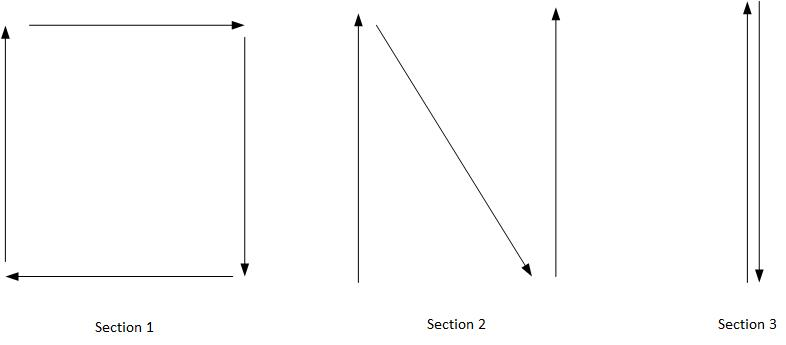
\includegraphics[width=.6\textwidth]{basic_traversal.jpg}
		\caption{Basic traversal patterns for Test 1 and 2}
		\label{fig:traversal_patterns}
	\end{figure}

	\subsection*{Test 2}
	Similar to test 1, but using the way point system instead. The positions were queued up and released for traversal at the end. These results will be compared to see how the traversal methods differ. The hypothesis is that friction and inertia will play a major factor in the auto correction system built into the navigation code.
	
	\subsection*{Test 3}
	This section differs from the first two as it introduces obstacles into the system. Since the beginning of this project, it was decided that path finding would play a major roll in having the robot cars figure out fast and efficient paths through moving and non-moving obstacles. Due to time constraints and limited space, only static obstacles were used. In addition, the equipment hadn't arrived for room scanning to be readily available, thus a measuring tape was used to help guess the dimensions and avoidance boundaries of these obstacles.
	\\
	These tests were broken up into two main categories, Test - 3A for a convex obstacle, and Test - 3B for a concave obstacle.
	
	\subsubsection*{Test 3 - A}
	This pattern flows around a central obstacle. The first section is single direction, the second is bidirectional. (figure\ref{fig:convex_travesal})
		\begin{figure}
			\centering
			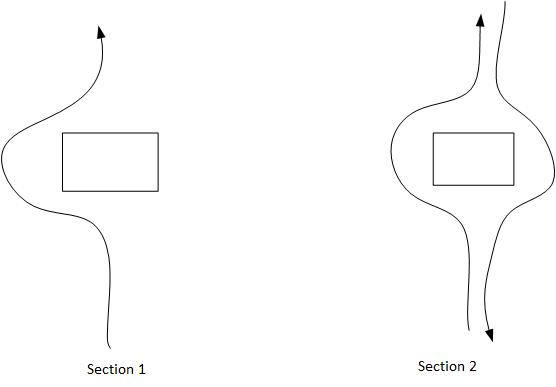
\includegraphics[width=.6\textwidth]{convex_traversals.jpg}
			\caption{Traversal pattern for Test 3A}
			\label{fig:convex_travesal}
		\end{figure}
	\subsubsection*{Test 3 - B}
	This pattern uses the A* search in a more complex manner, it travels around the corner of the L shape and to the destination, the second destination is ordering it to end up back where it started.(figure\ref{fig:concave_travesal})
		\begin{figure}
			\centering
			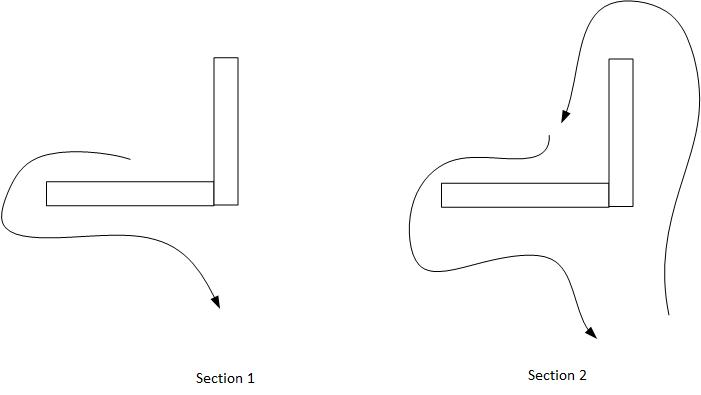
\includegraphics[width=.6\textwidth]{concave_traversals.jpg}
			\caption{Traversal pattern for Test 3B}
			\label{fig:concave_travesal}
		\end{figure}
	
	
	\section*{Data Analysis}
	Although the tests are broken into 3 sections, we'll only analyze Test section 1 for the comparison data, and sections 2 and 3 will be taking a look at just the behavioral aspects.
	
	This is done because the way point system wasn't set up for the Unity simulation, and neither were the obstacle system. These would've been trivial to do, but due to time constraints, the focus was shifted towards the VR controlled physical system instead.
	
	\subsection*{Visualized Results for Test Section 1}
	In figure \ref{fig:vis_comp_t1_1}, the motion vectors recorded in the log file is parsed and sorted into a csv file for graphing and visualizing. Unity supports debug drawing, so that API was used to draw the vectors in the game editor. The lines don't represent each delta time, which could be represented with various lengths if distance deltas were taken, but that feature was skipped for this portion due to time constraints.
	\\
	The visual comparison of test 1 - 1 shows a relatively accurate movement system. Where the Unity model on the right used in game floating point, rigid body physics, whereas the the model on the left represents the actual path traversed in Ruben's kitchen. The path of the VR robot car differers in the sense that rotation and maneuver could not be done simultaneously since it is the difference in rotation speed on the wheel motors that cause the turn. This was an oversight on the design of the API and control system of the Unity model, but nonetheless achieved a contrast of what game logic can do for both models.
	\\
	The 'fanning pattern can be seen in both, but more visible in the orange VR version. The robot car had crossed a specified threshold, thus causing to stop and rotate to an acceptable degree separation threshold from its target. The robot then was instructed to continue moving forward. All the operator had to do in this test was mark the four corners of the blue square, and both of these robots would attempt to reach each way point.
	\\
	On a high level note, this presents a way for robots to achieve various tasks using in game logic to model real world goals and heuristics. For example, if this were a package delivery service in a building, this car would have little trouble reaching its destination unless it had some serious obstructions.

		\begin{figure}
			\centering
			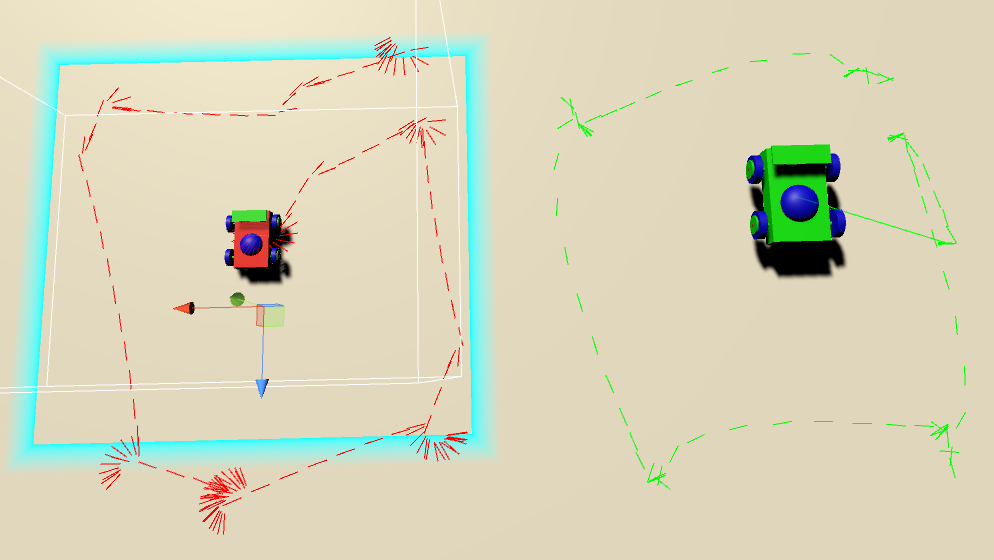
\includegraphics[width=.6\textwidth]{car_motion_vector_T1_1.png}
			\caption{Motion vectors for test 1 - 1}
			\label{fig:vis_comp_t1_1}
		\end{figure}
	In figure \ref{fig:vis_comp_t1_2}, the N shape was used for traversal. Each point on the path was sent to the robot one by one until it reached the position. This was done a couple of times to see how the robot would traverse on the way back.
		\begin{figure}
			\centering
			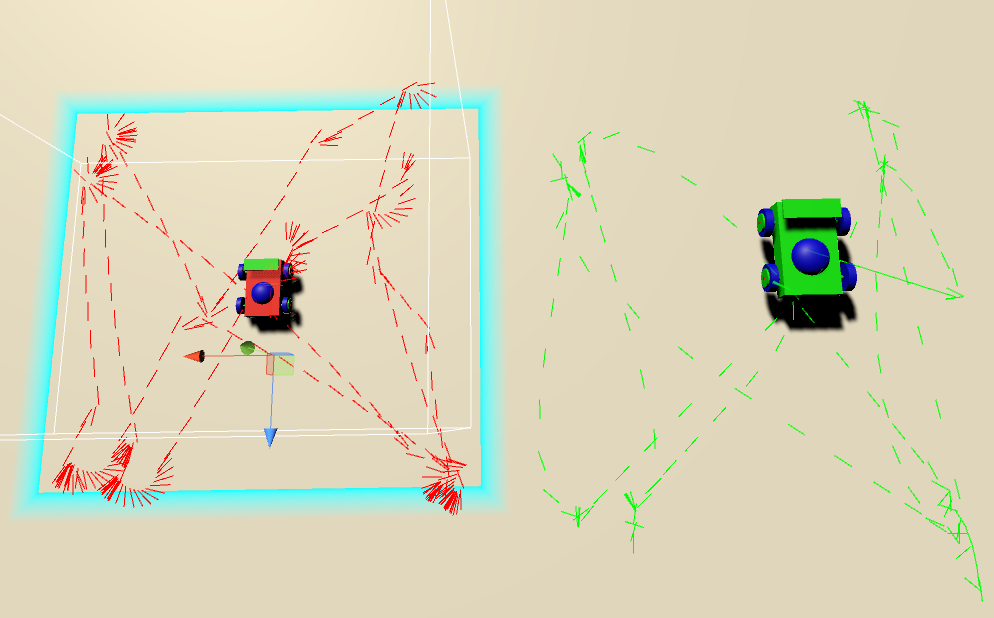
\includegraphics[width=.6\textwidth]{car_motion_vector_T1_2.png}
			\caption{Motion vectors for test 1 - 2, the N shape was traversed multiple times, producing an X like pattern instead}
			\label{fig:vis_comp_t1_2}
		\end{figure}
	In the last section of our clean paths test was the back and forth traversal in figure \ref{fig:vis_comp_t1_3}.
		\begin{figure}
			\centering
			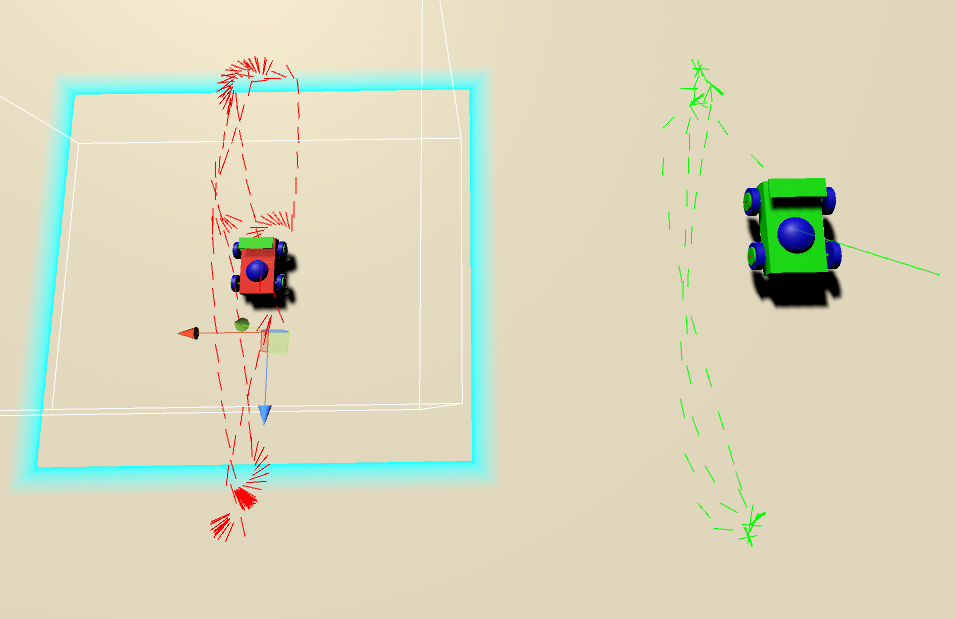
\includegraphics[width=.6\textwidth]{car_motion_vector_T1_3.png}
			\caption{The back and forth path. The green straight line in the corner of the car is from the initialization of the system.}
			\label{fig:vis_comp_t1_3}
		\end{figure}
	\subsection*{Graphed Results for Test 1}
	
	\subsection*{Way point Results for Test 2}
	
	\subsection*{Obstacle avoidance, A* search Results for Test 3}
	
	
	\section*{Conclusion}
	TODO: Summarize what actually happened, how well the system behave, performance measures in terms of response time.
	
	\section*{Future work}
	TODO: work on this in the future!
	
	\section*{REFERENCES}
	\begin{thebibliography}{99}
		
		\bibitem{hack1}{Cameron Coward, ''HTC Vive Gives Autonomous Robots Direction'',\url{http://hackaday.com/2016/08/23/htc-vive-gives-autonomous-robots-direction/},2016.}
		
			
		\bibitem{gizmodo1}{Sean Buckley, ''This Is How Valve?s Amazing Lighthouse Tracking Technology Works'',\url{http://gizmodo.com/this-is-how-valve-s-amazing-lighthouse-tracking-technol-1705356768},2016.}
		
	
		\bibitem{techradar1}{Jon Porter, ''This Is How Valve?s Amazing Lighthouse Tracking Technology Works'',\url{http://www.techradar.com/news/htc-vive-2-release-date-news-and-rumors}, 2017.}
		
		\bibitem{Bugalia}{Nishant Bugalia et. al., ''Immersive environment for robotic tele-operations'', 2015.}
		
		
		\bibitem{Codd-Downey}{Robert Codd-Downey and Michael Jenkin, ''Crime Scene Robot and Sensor Simulation'', 2009.}
		
		
	\end{thebibliography}
\end{document}
